\documentclass[a4paper]{article}
\usepackage[utf8]{inputenc}
\usepackage{draculatheme}
\usepackage{graphicx}
\usepackage{color}
\usepackage{nopageno}
\usepackage{fontawesome}
\usepackage[export]{adjustbox}

\usepackage[a4paper, total={7in, 11in}]{geometry}
\graphicspath{ {./} }
\title{Project 1 Submission}
\author{Chaitanya Sharma}
\date{January 2023}


\begin{document}
\begin{abstract}
    This is the design document of Chaitanya Sharma 
    for Project 1 for ECE 250's Winter 2023 offering.
\end{abstract}
\section{Class Structure}
    My program consisted of two major classes, namely {\color{draculapurple}VarDataNode} and 
    {\color{draculapurple}CalcLinkedList} and two independant functions, 
    one of which is obviously the {\color{draculapurple}main} function, and the other being a type 
    bool function {\color{draculapurple}printStatus} function. I've tested all edge test cases possible and also used the test cases provided by the jekelautograder on https://github.com/JZJisawesome/ece250-testcases
    \newline
    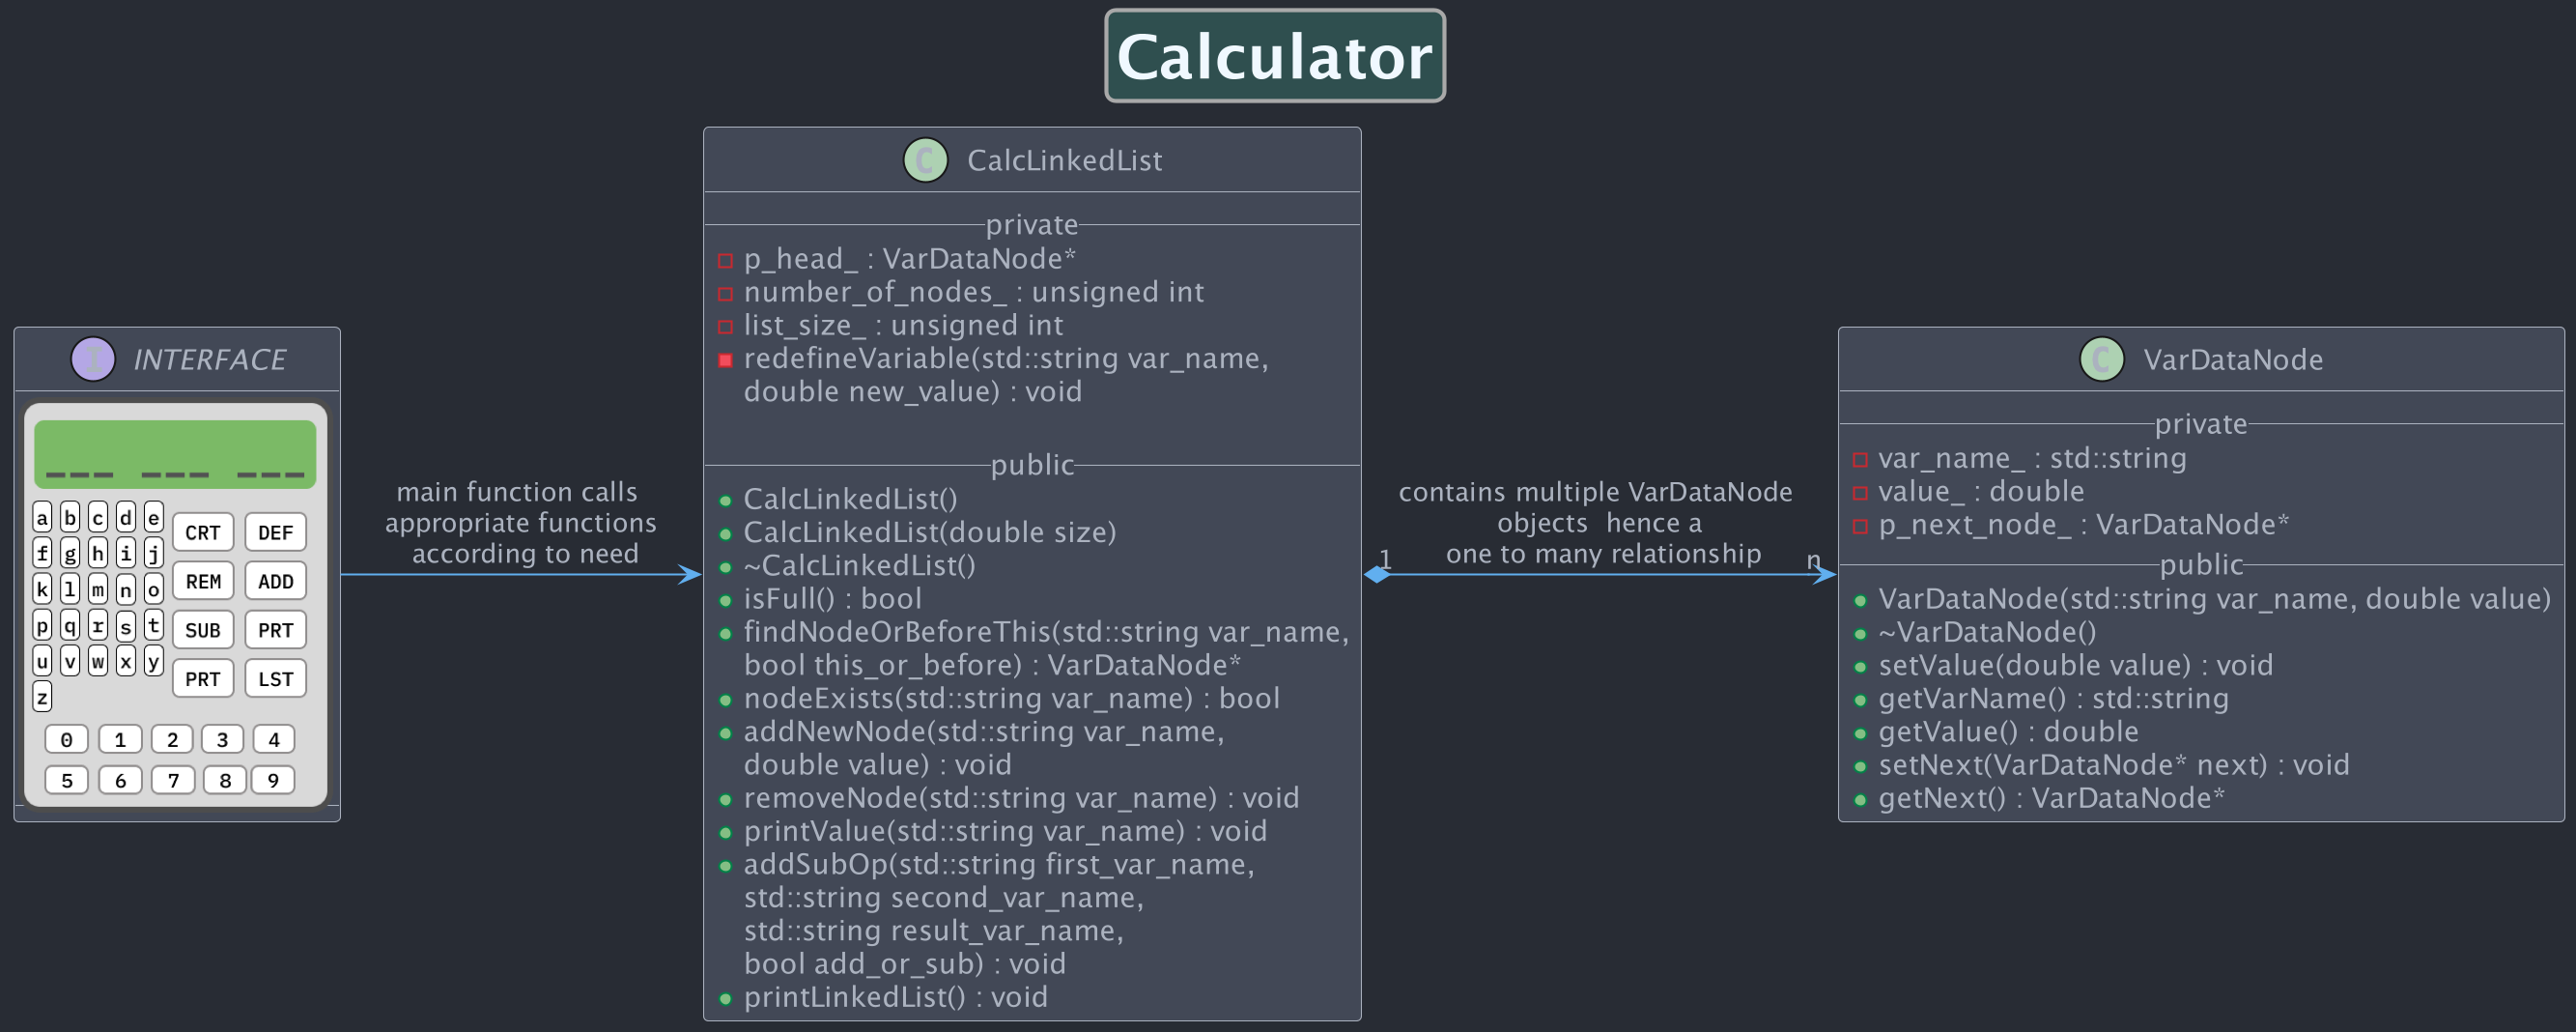
\includegraphics[scale=0.18, center]{Calculator.png}
    \subsection{\color{lightgray}Independant Functions}
    \subsubsection{{\color{orange}void} {\color{draculapurple}printStatus}({\color{orange}bool} {\color{yellow} status})}
    In this design document I will be going according to the order of my 
    code as well as sometimes the importance, hence since we're starting with the main file, the printStatus 
    function is a function which I created to reduce the cluttering of my 
    code due to repetitive usage of std::cout<<"success"<<std::endl; 
    and the opposite, and it runs in {\color{lightblue}O(1)} 
    since console output is one clock cycle.
    \subsubsection{{\color{orange} int} \color{draculapurple}main()}
    The main function is the entry point of my program, and it uses the 
    parsing structure which I borrowed and understood from what our Lab Instructor showed 
    in the vide HowToParseInGeneral on LEARN.

    It runs in {\color{lightblue}O(n)}, as it is a while loop which runs until there are 
    inputs, and then the input is disected into command conditions like 
    CRT, DEF, etc. Then, if the conditions provided to us in the table of 
    the project descriptions are true, and the program succeeds in 
    accomplishing the task given, it uses the {\color{draculapurple}printStatus} 
    to provide the output of success, and vica versa. But since it runs the program itself, 
    we discard its runtime costs for calculation and theory of runtime purposes, 
    as it is the base of the program itself.
    \subsection{{\color{orange}class} {\color{draculapurple}VarDataNode}}
    This class is the class which is used to create the nodes of the Linked List, 
    hence it needs to store all the data needed in a node, according to use case, 
    which in our case is the variable name{\color{orange}(as a string)}, and the value of the 
    variable{\color{orange}(as a double)}, and a pointer, since this is supposed to be private information, 
    they're designated privately as var\_name\_, value\_ and p\_next\_node\_ respectively. 
    Also, they have their own setters and getters{\color{lightblue}(all in O(1))}, 
    but in the case of the variable name, there's no setter since I didn't find 
    any use case for it. 
    
    Though we're not asked to redefine a variable's value anywhere explicitly, i
    n the design document, it is given in context of addition and subtract operations, 
    that the result variable needs to exist already, meaning that the setter 
    for the variable value is needed. All other setters and getters are 
    necessary for the functioning of the linked list. 
    \subsubsection{\color{draculapurple}CONSTRUCTOR AND DESTRUCTOR}
    As there's no use of a no-value constructor, but I have included a value-init constructor, 
    which initializes appropriate values {\color{lightblue}(in O(1))}.
    I have used C++'s internal feature of a Default Destructor, 
    by equating the destructor declaration to default, since this a very 
    simple and and independant class which does not allocate anythin on the heap itself. 
    \subsection{{\color{orange}class} {\color{draculapurple}CalcLinkedList}}
    On the subject of {\color{LimeGreen}head\_} pointer, it is the most crucial part of a linked list, 
    also, the {\color{LimeGreen}list\_size\_} which is required for initializing 
    the list with a defined size is also kept private and due to no 
    need of modifying/accessing them outside of this class, there's no setters/getters.

    I added the {\color{LimeGreen}number\_of\_nodes\_} private variable to keep 
    track of the number of nodes in the list, as it is a given requirement 
    to not let the user define more nodes than the original size specified, 
    and at some advanced level, it would be more computationally sound to keep 
    track rather than calculate it.

    I also added a redefineVariable private function, which is 
    used only in the add and subtract functions as they assign the result value 
    to an already-defined variable.
    \subsubsection{\color{draculapurple}CONSTRUCTOR}
    I've added a no-value constructor, which initializes the {\color{LimeGreen}head\_} and 
    {\color{LimeGreen}list\_size\_} to nullptr and 0 respectively, and the {\color{LimeGreen}number\_of\_nodes\_} to 0.
    A value-init constructor, which initializes the {\color{LimeGreen}head\_} to nullptr, 
    {\color{LimeGreen}list\_size\_} to the size given, and {\color{LimeGreen}number\_of\_nodes\_} to 0. "CRT"
    \subsubsection{\color{draculapurple}DESTRUCTOR}
    Since memory leak is a major grading ground of this project, 
    hence even though small, but this was one of the most focus-requiring 
    portion of my code, I create a temp pointer which starts at head and deletes 
    it and moves on to another node until it sees a {\color{LightPink}nullptr}. "END"
    \subsubsection{{\color{orange}bool} {\color{draculapurple}isFull}()}
    This function just returns the result of the comparison of the 
    {\color{LimeGreen}number\_of\_nodes\_} and {\color{LimeGreen}list\_size\_} through the equality operator.
    \subsubsection{{\color{orange}VarDataNode*} 
    {\color{draculapurple}findNodeOrBeforeThis}
    ({\color{orange}std::string} var\_name, \newline
    {\color{orange}bool} true\_is\_this\_false\_is\_before\_this)
    \faStar~~{\color{awesome}a special feature of my code}~~\faStar}
    A problem was running while loop in many of my functions, an iterative finder 
    function would be not intuitive since removeNode would still traverse and 
    the other three function {\color{draculapurple}printValue}, {\color{draculapurple}addSubOp} and 
    {\color{draculapurple}nodeExists} wouldn't, hence it was hard, BUT I COULD make a function which found the node before the 
    node to be found, according to a condition, where the removeNode function would 
    directly get the previous node to bypass the node to be deleted using a bool 
    parameter {\color{GoldenYellow}false}, while the other functions use {\color{GoldenYellow}true}
    to get the pointer to that exact node. I take in the second parameter to decide 
    whether the function is to return the pointer for node for variable name given, 
    or the pointer for the node before the node for variable name given.
    In this function, I am basically exploiting the fact that 
    {\color{lightblue}O(n+1) is still == O(n)} as it uses a traversal loop to find the node.
    \subsubsection{{\color{orange}bool} {\color{draculapurple}nodeExists}
    ({\color{orange}std::string} var\_name )}
    This function just returns the result of the comparison of the result from {\color{draculapurple}findNodeBeforeThis} with the arguments of the variable requested and true
    \subsubsection{{\color{orange}void} {\color{draculapurple}addNewNode}
    ({\color{orange}std::string} var\_name, {\color{orange}double} value)}
    This function first allocates a new VarDataNode on the heap, 
    and then sets its next pointer to the head pointer, and reassigns the 
    {\color{LimeGreen}head\_} pointer to the new node, and then increments 
    the {\color{LimeGreen}number\_of\_nodes\_} by 1. "DEF"
    \subsubsection{{\color{orange}void} {\color{draculapurple}removeNode}({\color{orange}std::string} var\_name)}
    For the head node, I just set the {\color{LimeGreen}head\_} pointer to the next node, 
    and for all else, I get the pointer to the node before the node to be deleted, and 
    then sets its next pointer to the next node of the node to be deleted, and then 
    finally deletes the node at the address from temp pointer. The runtime of this 
    function is {\color{lightblue}O(n)} since it uses the {\color{draculapurple}findNodeOrBeforeThis} function for traversal. 
    "REM"
    \subsubsection{{\color{orange}void} {\color{draculapurple}printValue}({\color{orange}std::string} var\_name)}
    This function uses the {\color{draculapurple}findNodeOrBeforeThis} function to 
    get the pointer to the node with the variable name given, and then uses 
    {\color{orange}std::cout} to print the value of that node by using 
    {\color{draculapurple}getValue} function. "PRT"
    \subsubsection{{\color{orange}void} {\color{draculapurple}addSubOp}
    ({\color{orange}std::string} first\_var\_name, 
    {\color{orange}std::string} second\_var\_name,\newline 
    {\color{orange}std::string} result\_var\_name), 
    {\color{orange}bool} add\_or\_sub}
    This function uses the {\color{draculapurple}findNodeOrBeforeThis} with function 
    to get the value of the operands, then according to the boolean parameter, it adds
    or subtracts the two values if true or false respectively and then assigns the result. 
    The runtime of this function is {\color{lightblue}O(n)} since there are only sequential 
    while loops and not nested ones and that too due to calling {\color{draculapurple}findNodeOrBeforeThis} function. "ADD" AND "SUB"
    \subsubsection{{\color{orange}void} {\color{draculapurple}printLinkedList}() {\color{awesome}CONVENIENCE FUNCTION:} {\color{yellow}beautifully prints the linked list}} 
    "LST"
\end{document}